\documentclass[10pt,a4paper]{article}
\usepackage[a4paper, left=3cm, right=3cm, top=3cm, bottom=3cm, headsep=10mm, footskip=12mm]{geometry}
\usepackage[T1]{fontenc}
\usepackage[ngerman, english]{babel}    % mehrsprachiger Textsatz
% babel: letzte Sprache in Optionen zeigt die Sprache des Dokumentes
% und kann durch den Befehl \selectlanguage{} geaendert werden
% Passen Sie die Optionen des babel-Paketes nach Bedarf an!
\usepackage{float}
\usepackage{graphicx}
\usepackage{url}
\usepackage{pdflscape}
\usepackage{mathtools}
\usepackage{amssymb, amsmath, amstext}
\usepackage{amsthm}
\usepackage{xcolor}
\usepackage{nameref}
\usepackage{siunitx}
\usepackage{makecell}
\usepackage{hyperref}
\usepackage{enumitem}
\usepackage[superscript,biblabel]{cite}
\usepackage{caption}
\usepackage{subcaption}
\usepackage{tabularx} 			% Tabellen erzeugen
\usepackage{multirow}			 % Zeilen in Tabellenbearbeitung
\usepackage{multicol} 			% Spalten in Tabellenbearbeitung 
\usepackage{lmodern}                        % Ersatz fuer Computer Modern-Schriften 
\usepackage{amsmath}                                           % zum besseren Aussehen am Bildschirm
\usepackage{booktabs} % für schönere Tabellen
\usepackage{sidecap}
\usepackage{rotating} % für die Landscape-Umgebung
\usepackage{afterpage}
\definecolor{Bluetitle}{HTML}{1F3864}
\definecolor{softbluetitle}{HTML}{274D7E}
\definecolor{Greyish}{HTML}{5A5A5A}
\renewcommand{\refname}{Reference}
\usepackage{array,multirow}
\newcommand{\specialcell}[2][c]{%
	\begin{tabular}[#1]{@{}c@{}}#2\end{tabular}}




\begin{document}
	
	\begin{titlepage}
		\begin{center}
			\begin{figure}[h!tbp]
				
\includegraphics[width=\linewidth]{HUlogo.PNG}
			\end{figure}
			\vspace*{2 cm}
			
			\textcolor{Bluetitle}{\textbf{\huge Atmung und Gährung}}\par
			
			\vspace*{2cm}
			
			\textcolor{Greyish}{\textbf{Versuchsdurchführende}}\par
			\textcolor{Greyish}{Oscar Moore (634083)}\par
			\textcolor{Greyish}{Fridolin Rehnig (625757)}\par
			\textcolor{Greyish}{Philipp Kunze (625468)}\par
			\textcolor{Greyish}{Daniel Kollenkirchen (625426)}\par
			\textcolor{Greyish}{Huyen Anh Nguyen (572309)}\par
			
			\vspace*{0.5cm}
			\textcolor{Greyish}{\textbf{Versuchsort}}\par
			\textcolor{Greyish}{Campus Nord, Haus 9}\par
			\textcolor{Greyish}{R2001}\par
			\vspace*{0.5cm}
			\textcolor{Greyish}{\textbf{Versuchsbetreuer}}\par
			\textcolor{Greyish}{Dr. Boris Hedtke}\par
			
			\vspace*{2 cm}
			
			\textcolor{Greyish}{02. Juli 2024}\par
			
			
			
			
		\end{center}
	\end{titlepage}
	
	\tableofcontents
	
	\section{Einführung}	

	
	
	\section{Material und Methode}

	
	\section{Ergebnis}
	\subsection{Aerobe und anaerobe Glucoseverbrauch}
	Es wurde 1.8g Glucose in 250mL Medium gelöst, welches eine Anfangskonzentration von 40mM ergibt.
	
		\begin{table}[H]
		\centering
		\caption{Glucoseverbrauch von Backhefe in aerobe und Anaerobe Bedingungen. Glucoseverbrauch wurde nach den bei farbliche betrachtung von den Skala in Figure \ref{fig: Glucoseverbrauch} abgelesen }
		\label{tab:glucoseverbrauch anareob und aerob}
		\begin{tabular}{ccc}
			\toprule
			\multirow{2}{*}{t in min} & \specialcell[t]{Glucoseverbrauch bei \\ aerobe Bedingung in mM}& \specialcell[t]{Glucoseverbrauch bei \\anaerobe Bedingung in mM}\\
			\midrule
			10 & 111 & 55\\
			15 & 55 & 28\\
			20 & 14 & <14\\
			25 & 5.5 & 0\\
			\bottomrule
		\end{tabular}
	\end{table}	
	\subsection{Anaerobe Gährung}
	\subsection{Sauerstoffverbrauch und cyanidresistente Atmung}
		\begin{table}[H]
		\centering
		\caption{Sauerstoff- und Glucoseverbrauch von Backhefe und BY2-Pflanzenzellen in anaeroben Bedingungen mit und ohne Zugabe von Kaliumcyanid.}
		\label{tab:O2verbrauch und CN}
		\begin{tabular}{ccc}
			\toprule
			& $O_2$-Verbrauch in $\mu$g/L min g& Glucose-Verbrauch in mM/ min g\\
			\midrule
			Hefe ohne KCN & 311.4 & 3.244 $\cdot$ 10$^{-3}$\\
			Hefe mit KCN & 54.42& 5.669 $\cdot$ 10$^{-7}$\\
			& & \\
			BY2 ohne KCN & 96.36 & 2.868 $\cdot$ 10$^{-8}$\\
			BY2 mit KCN & 132.8& 3.954 $\cdot$ 10$^{-8}$\\
			\bottomrule
		\end{tabular}
	\end{table}	
	
	\section{Diskussion}

	\section{Anhang}
	\subsection{Rohdaten}
		\begin{figure}[H]
		\centering
		\begin{subfigure}[b]{0.4\textwidth}
			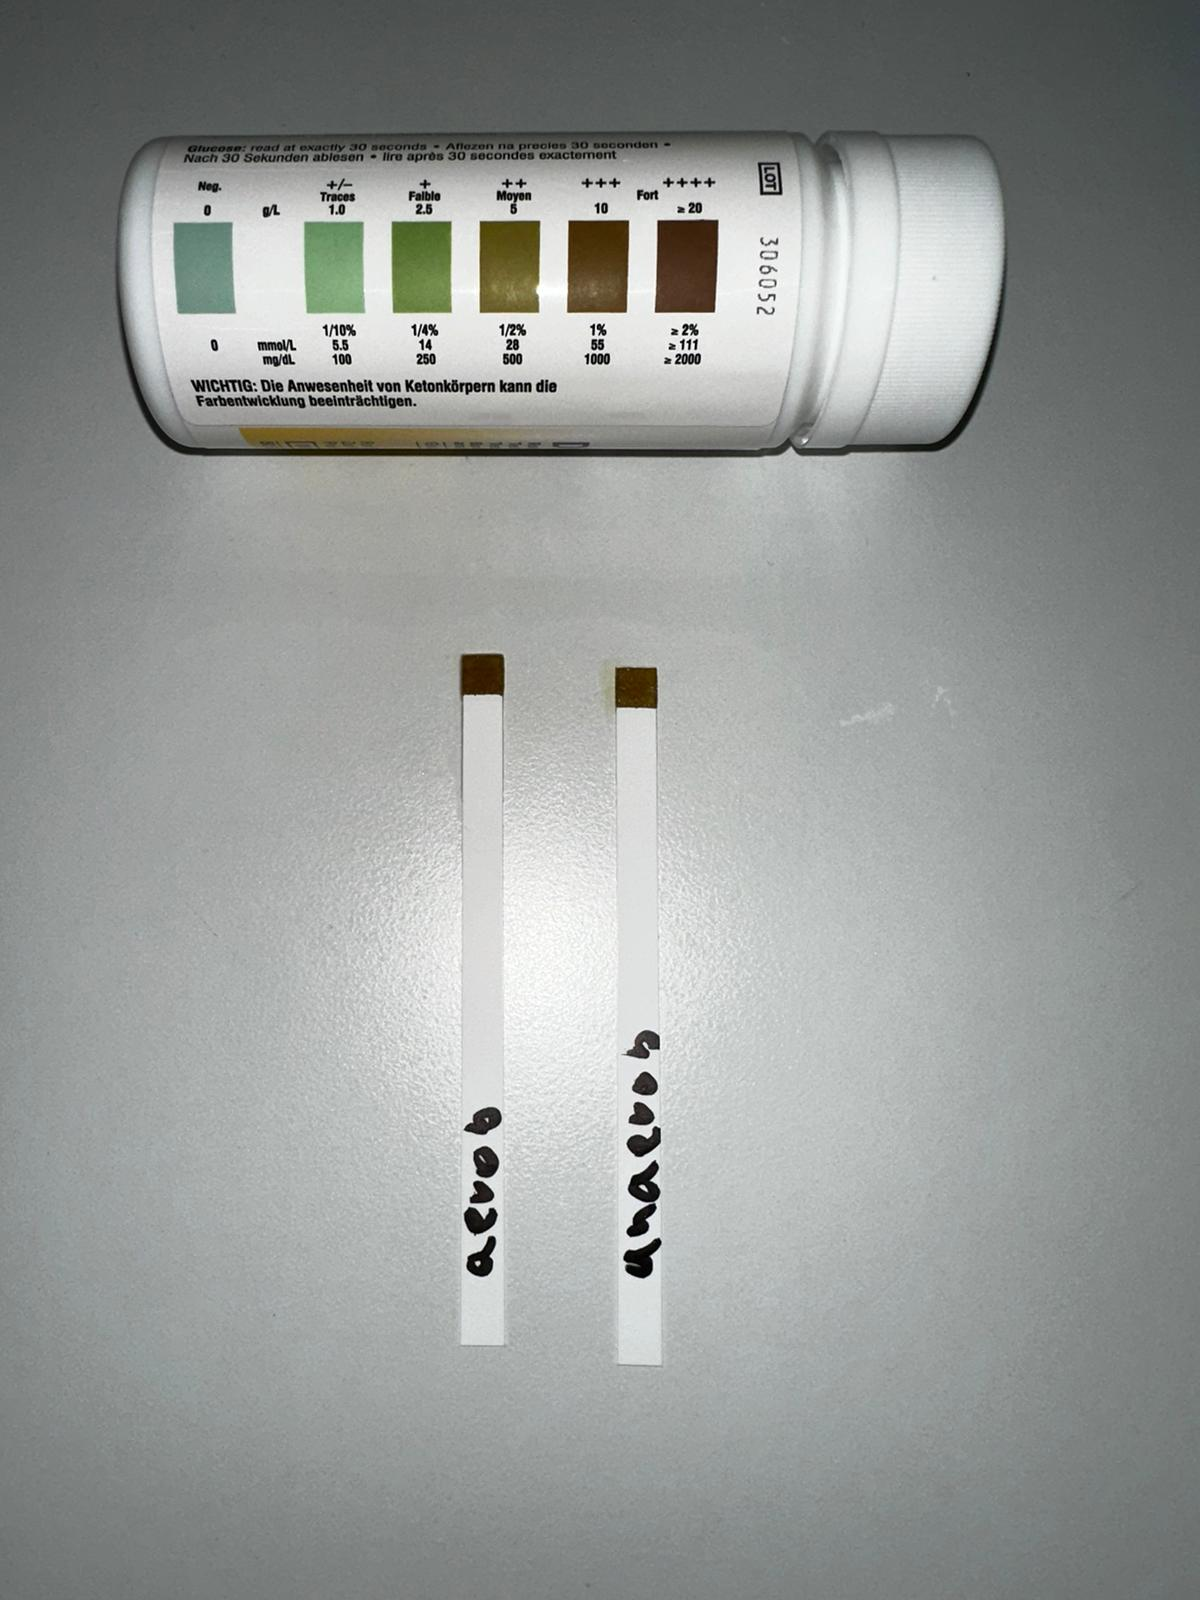
\includegraphics[width=\textwidth]{PHOTO-2024-07-04-23-51-30.jpg}
			\caption{10 Minuten}
			\label{fig:10min}
		\end{subfigure}
		\hfill
		\begin{subfigure}[b]{0.4\textwidth}
			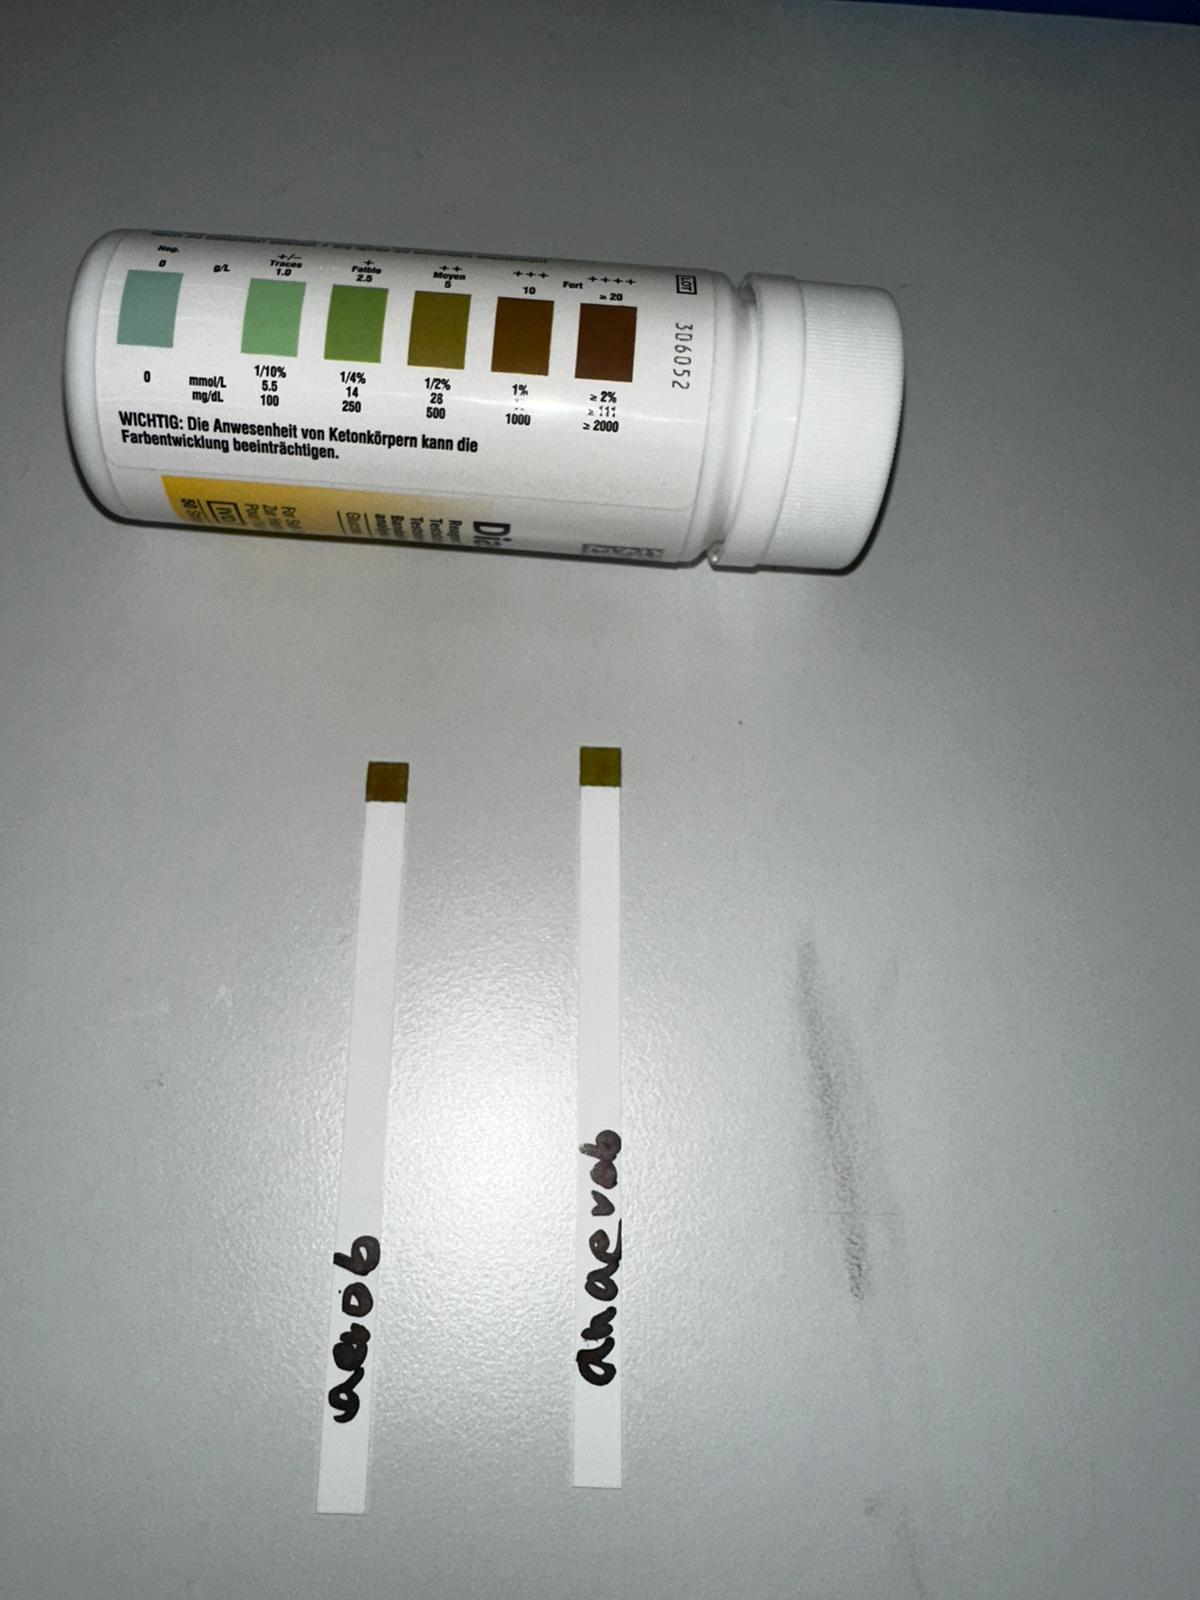
\includegraphics[width=\textwidth]{PHOTO-2024-07-04-23-51-29 2.jpg}
			\caption{15 Minuten}
			\label{fig:15 min}
		\end{subfigure}
		\begin{subfigure}[b]{0.4\textwidth}
			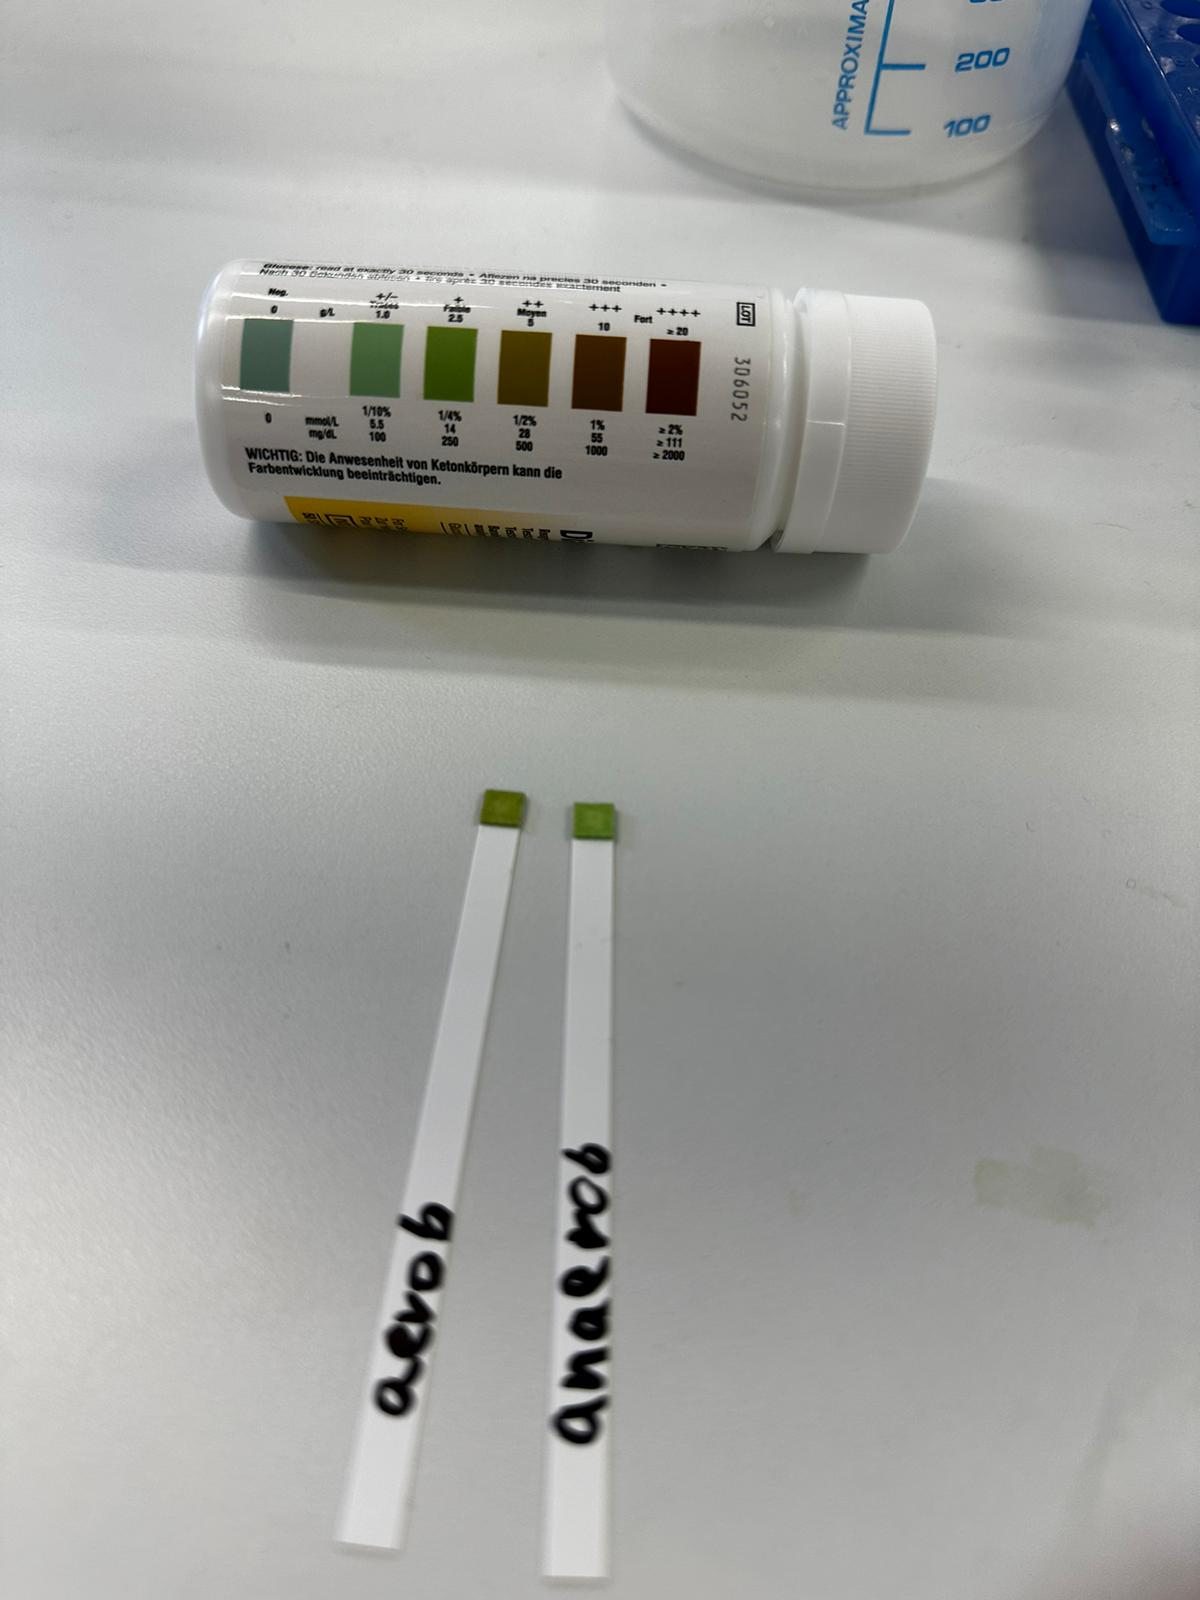
\includegraphics[width=\textwidth]{PHOTO-2024-07-04-23-51-28 2.jpg}
			\caption{20 Minuten}
			\label{fig:20 min}
		\end{subfigure}
		\hfill
		\begin{subfigure}[b]{0.4\textwidth}
			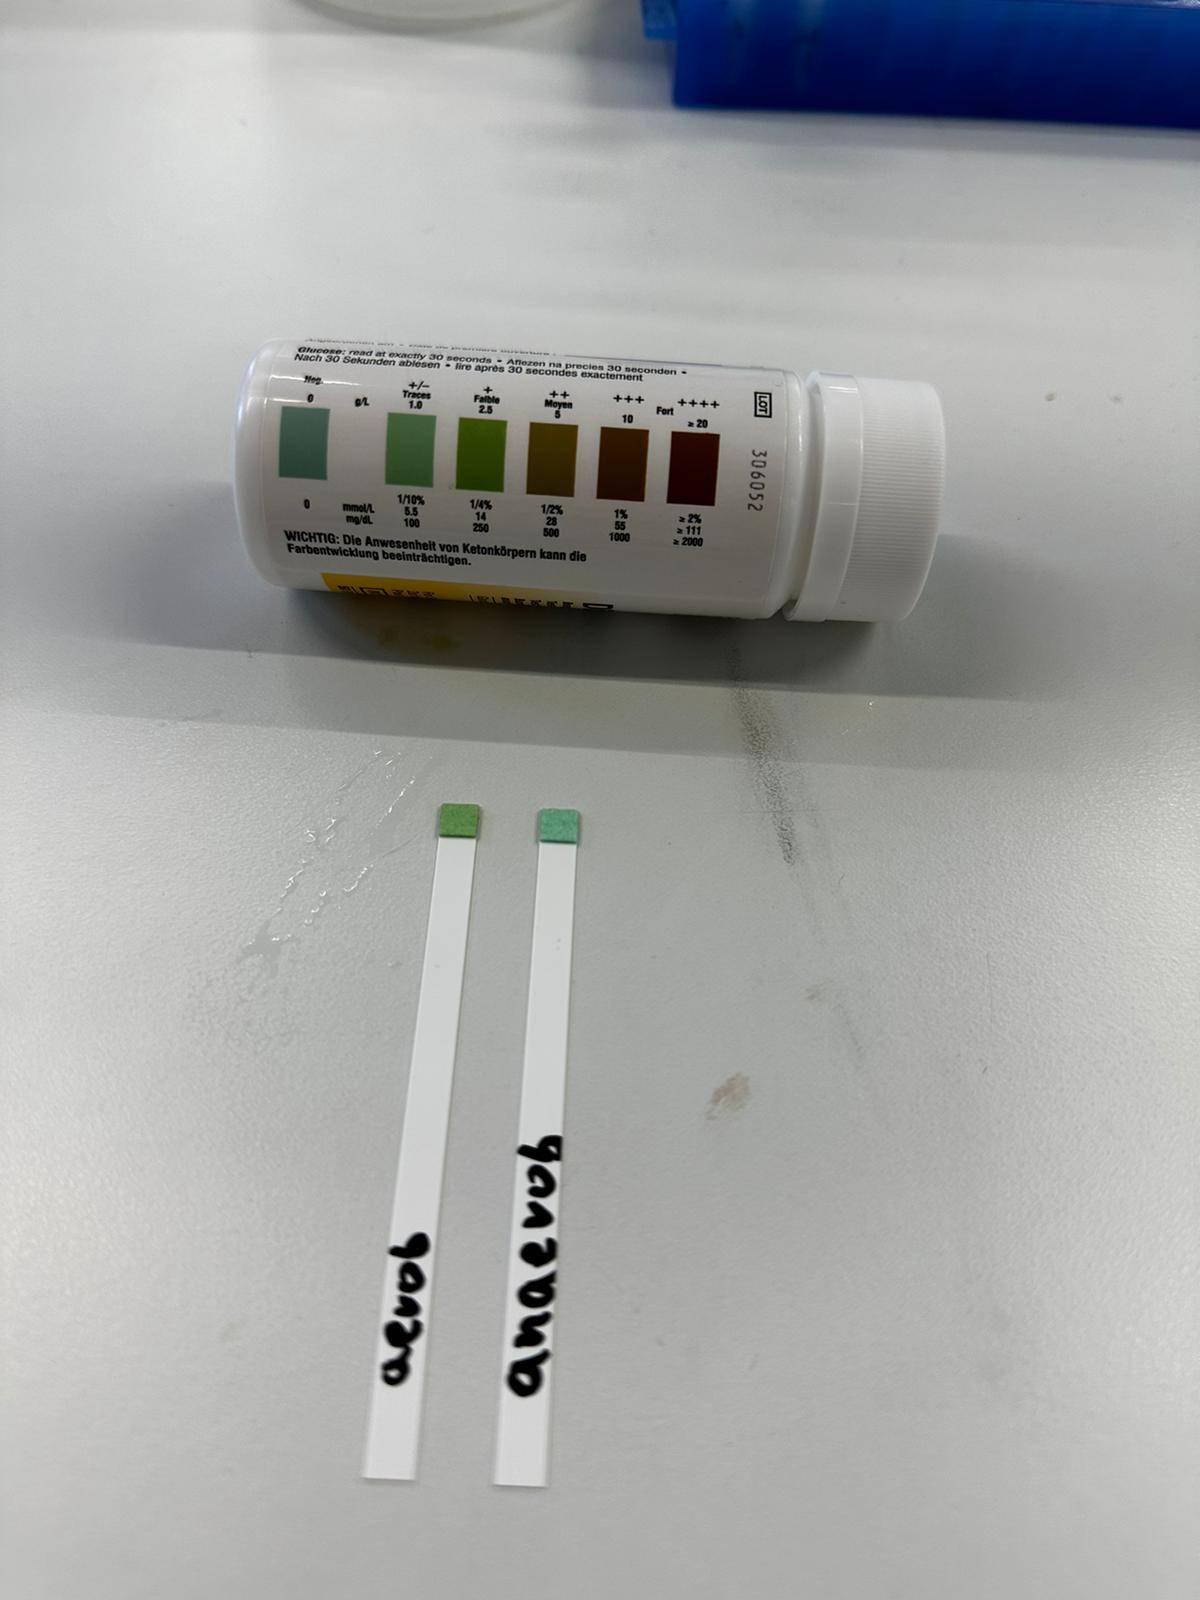
\includegraphics[width=\textwidth]{PHOTO-2024-07-04-23-51-29.jpg}
			\caption{25 Minuten}
			\label{fig:25 min}
		\end{subfigure}
		\caption{Teststreifen nach 10, 15, 20, 25 Minuten in den Backhefe-Lösung bei aerobe und anaerobe Bedingungen.}
		\label{fig: Glucoseverbrauch}
	\end{figure}
			
	\begin{table}[H]
		\centering
		\caption{Sauerstoffkonzentration von 0.52g Backhefe in einer anaeroben Bedingung.}
		\label{tab:O2 Backhefe ohne KCN}
		\begin{tabular}{cc}
			\toprule
			t in min& ß($O_2$) in mg/L\\
			\midrule
			1.30 & 5.90\\
			2.00 & 5.0\\
			2.30 & 5.34\\
			3.00 & 5.07\\
			3.30 & 4.84 \\
			4.00 & 4.54 \\
			4.30 & 4.30 \\
			5.00 & 4.03 \\
			6.00 & 3.50 \\
			6.30 & 3.23\\
			7.00 & 2.95\\
			7.30 & 2.66\\
			8.00 & 2.38\\
			8.30 & 2.10 \\
			9.00 & 1.84\\
			9.30 & 1.56 \\
			10.00 & 1.29\\
			10.30 & 1.01\\
			11.00 & 0.74\\
			11.30 & 0.47\\
			12.00 & 0.21\\
			12.30 & 0.05\\
			13.00 & 0.00\\			
			\bottomrule
		\end{tabular}
	\end{table}	
	
	\begin{table}[H]
		\centering
		\caption{Sauerstoffkonzentration von 0.52g Backhefe in einer anaeroben Bedingung und Zugabe von 2.4mL 10mM Kaliumcyanid.}
		\label{tab:O2 Backhefe mit KCN}
		\begin{tabular}{cc}
			\toprule
			t in min& ß($O_2$) in mg/L\\
			\midrule
			0.30 & 5.85\\
			1.00 & 5.56\\
			1.30 & 5.49\\
			2.00 & 5.49\\
			2.30 & 5.19 \\
			3.00 & 5.12 \\
			3.30 & 5.08 \\
			4.00 & 5.03\\
			4.30 & 4.97\\
			5.00 & 4.94 \\
			5.30 & 4.89\\
			6.00 & 4.84\\
			6.30 & 4.81\\
			7.00 & 4.77 \\
			7.30 & 4.72\\
			\bottomrule
		\end{tabular}
	\end{table}	
	
	\begin{table}[H]
		\centering
		\caption{Sauerstoffkonzentration von 5.25g BY2-Zellen in einer anaeroben Bedingung.}
		\label{tab:O2 BY2 ohne KCN}
		\begin{tabular}{cc}
			\toprule
			t in min& ß($O_2$) in mg/L\\
			\midrule
			0.30 & 8.09\\
			1.00 & 8.03\\
			1.30 & 7.96\\
			2.00 & 7.93\\
			2.30 & 7.87 \\
			3.00 & 7.83 \\
			3.30 & 7.82 \\
			4.00 & 7.73\\
			4.30 & 7.69\\
			5.00 & 7.64 \\
			\bottomrule
		\end{tabular}
	\end{table}	
	
	\begin{table}[H]
		\centering
		\caption{Sauerstoffkonzentration von 5.25g BY2-Zellen in einer anaeroben Bedingung und Zugabe von 2.4mL 10mM Kaliumcyanid.}
		\label{tab:O2 BY2 mit KCN}
		\begin{tabular}{cc}
			\toprule
			t in min& ß($O_2$) in mg/L\\
			\midrule
			0.30 & 7.61\\
			1.00 & 7.56\\
			1.30 & 7.48\\
			2.00 & 7.41\\
			2.30 & 7.36 \\
			3.00 & 7.30 \\
			3.30 & 7.23 \\
			4.00 & 7.16\\
			4.30 & 7.08\\
			5.00 & 7.01 \\
			\bottomrule
		\end{tabular}
	\end{table}	
	
	
	
	
	\addcontentsline{toc}{section}{References}
	\bibliographystyle{plainurl}
	\nocite{*}
	\bibliography{Literatur}
	\newpage
	
	
\end{document}